% Created by tikzDevice version 0.12.3.1 on 2023-03-16 10:37:09
% !TEX encoding = UTF-8 Unicode
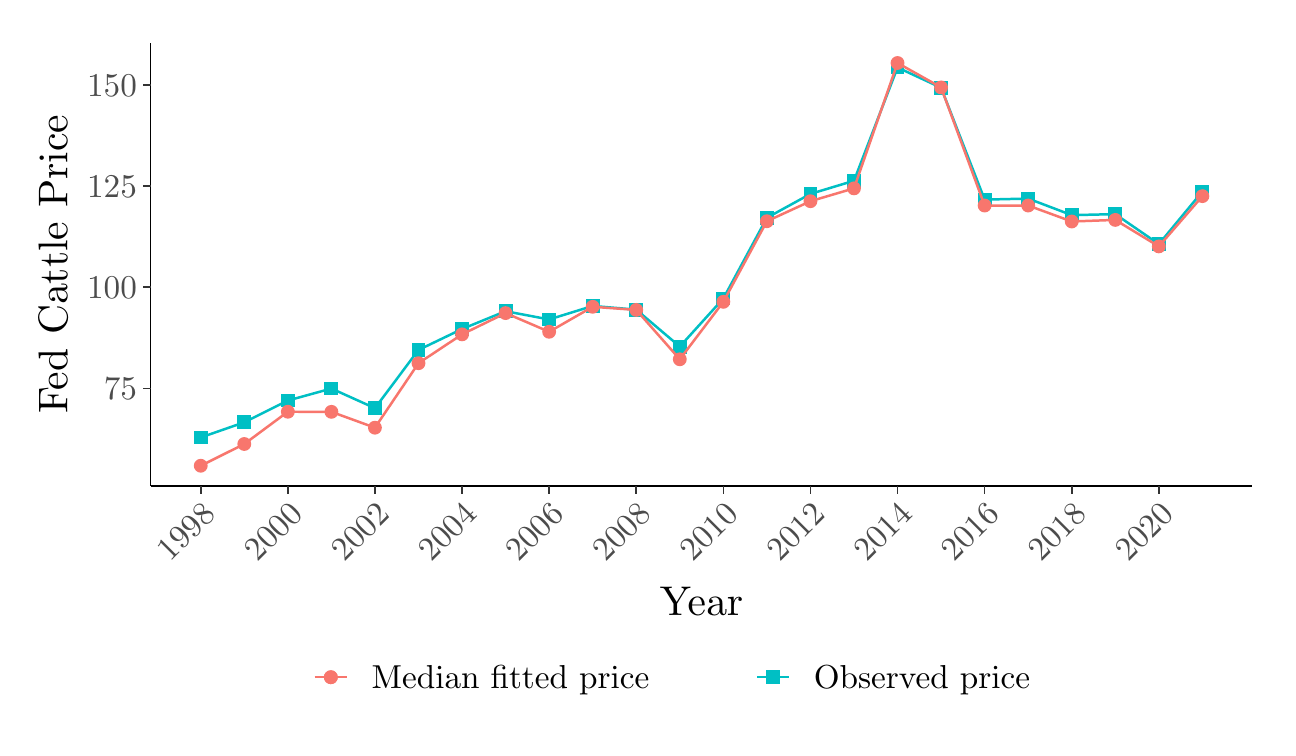
\begin{tikzpicture}[x=1pt,y=1pt]
\definecolor{fillColor}{RGB}{255,255,255}
\path[use as bounding box,fill=fillColor,fill opacity=0.00] (0,0) rectangle (448.07,252.94);
\begin{scope}
\path[clip] (  0.00,  0.00) rectangle (448.07,252.94);
\definecolor{drawColor}{RGB}{255,255,255}
\definecolor{fillColor}{RGB}{255,255,255}

\path[draw=drawColor,line width= 0.6pt,line join=round,line cap=round,fill=fillColor] (  0.00,  0.00) rectangle (448.07,252.94);
\end{scope}
\begin{scope}
\path[clip] ( 44.44, 87.36) rectangle (442.57,247.45);
\definecolor{fillColor}{RGB}{255,255,255}

\path[fill=fillColor] ( 44.44, 87.36) rectangle (442.57,247.44);
\definecolor{drawColor}{RGB}{0,191,196}

\path[draw=drawColor,line width= 0.9pt,line join=round] ( 62.54,104.86) --
	( 78.28,110.34) --
	( 94.01,118.20) --
	(109.75,122.54) --
	(125.48,115.45) --
	(141.22,136.48) --
	(156.96,144.05) --
	(172.69,150.48) --
	(188.43,147.50) --
	(204.17,152.38) --
	(219.90,151.05) --
	(235.64,137.69) --
	(251.38,155.08) --
	(267.11,184.23) --
	(282.85,192.87) --
	(298.59,197.62) --
	(314.32,238.55) --
	(330.06,231.24) --
	(345.79,190.81) --
	(361.53,191.18) --
	(377.27,185.20) --
	(393.00,185.56) --
	(408.74,174.73) --
	(424.48,193.73);
\definecolor{fillColor}{RGB}{0,191,196}

\path[fill=fillColor] ( 60.04,102.36) --
	( 65.04,102.36) --
	( 65.04,107.35) --
	( 60.04,107.35) --
	cycle;

\path[fill=fillColor] ( 75.78,107.84) --
	( 80.77,107.84) --
	( 80.77,112.84) --
	( 75.78,112.84) --
	cycle;

\path[fill=fillColor] ( 91.51,115.71) --
	( 96.51,115.71) --
	( 96.51,120.70) --
	( 91.51,120.70) --
	cycle;

\path[fill=fillColor] (107.25,120.05) --
	(112.25,120.05) --
	(112.25,125.04) --
	(107.25,125.04) --
	cycle;

\path[fill=fillColor] (122.99,112.96) --
	(127.98,112.96) --
	(127.98,117.95) --
	(122.99,117.95) --
	cycle;

\path[fill=fillColor] (138.72,133.98) --
	(143.72,133.98) --
	(143.72,138.97) --
	(138.72,138.97) --
	cycle;

\path[fill=fillColor] (154.46,141.55) --
	(159.46,141.55) --
	(159.46,146.54) --
	(154.46,146.54) --
	cycle;

\path[fill=fillColor] (170.20,147.98) --
	(175.19,147.98) --
	(175.19,152.98) --
	(170.20,152.98) --
	cycle;

\path[fill=fillColor] (185.93,145.00) --
	(190.93,145.00) --
	(190.93,149.99) --
	(185.93,149.99) --
	cycle;

\path[fill=fillColor] (201.67,149.88) --
	(206.66,149.88) --
	(206.66,154.88) --
	(201.67,154.88) --
	cycle;

\path[fill=fillColor] (217.41,148.55) --
	(222.40,148.55) --
	(222.40,153.55) --
	(217.41,153.55) --
	cycle;

\path[fill=fillColor] (233.14,135.19) --
	(238.14,135.19) --
	(238.14,140.19) --
	(233.14,140.19) --
	cycle;

\path[fill=fillColor] (248.88,152.59) --
	(253.87,152.59) --
	(253.87,157.58) --
	(248.88,157.58) --
	cycle;

\path[fill=fillColor] (264.62,181.73) --
	(269.61,181.73) --
	(269.61,186.73) --
	(264.62,186.73) --
	cycle;

\path[fill=fillColor] (280.35,190.37) --
	(285.35,190.37) --
	(285.35,195.37) --
	(280.35,195.37) --
	cycle;

\path[fill=fillColor] (296.09,195.12) --
	(301.08,195.12) --
	(301.08,200.12) --
	(296.09,200.12) --
	cycle;

\path[fill=fillColor] (311.82,236.05) --
	(316.82,236.05) --
	(316.82,241.05) --
	(311.82,241.05) --
	cycle;

\path[fill=fillColor] (327.56,228.75) --
	(332.56,228.75) --
	(332.56,233.74) --
	(327.56,233.74) --
	cycle;

\path[fill=fillColor] (343.30,188.31) --
	(348.29,188.31) --
	(348.29,193.31) --
	(343.30,193.31) --
	cycle;

\path[fill=fillColor] (359.03,188.68) --
	(364.03,188.68) --
	(364.03,193.67) --
	(359.03,193.67) --
	cycle;

\path[fill=fillColor] (374.77,182.70) --
	(379.77,182.70) --
	(379.77,187.69) --
	(374.77,187.69) --
	cycle;

\path[fill=fillColor] (390.51,183.06) --
	(395.50,183.06) --
	(395.50,188.06) --
	(390.51,188.06) --
	cycle;

\path[fill=fillColor] (406.24,172.23) --
	(411.24,172.23) --
	(411.24,177.23) --
	(406.24,177.23) --
	cycle;

\path[fill=fillColor] (421.98,191.24) --
	(426.97,191.24) --
	(426.97,196.23) --
	(421.98,196.23) --
	cycle;
\definecolor{drawColor}{RGB}{248,118,109}

\path[draw=drawColor,line width= 0.9pt,line join=round] ( 62.54, 94.64) --
	( 78.28,102.50) --
	( 94.01,114.16) --
	(109.75,114.12) --
	(125.48,108.39) --
	(141.22,131.69) --
	(156.96,142.12) --
	(172.69,149.80) --
	(188.43,143.05) --
	(204.17,152.08) --
	(219.90,150.95) --
	(235.64,133.11) --
	(251.38,153.87) --
	(267.11,183.00) --
	(282.85,190.23) --
	(298.59,194.88) --
	(314.32,240.17) --
	(330.06,231.35) --
	(345.79,188.67) --
	(361.53,188.67) --
	(377.27,182.90) --
	(393.00,183.47) --
	(408.74,173.90) --
	(424.48,192.06);
\definecolor{fillColor}{RGB}{248,118,109}

\path[fill=fillColor] ( 62.54, 94.64) circle (  2.50);

\path[fill=fillColor] ( 78.28,102.50) circle (  2.50);

\path[fill=fillColor] ( 94.01,114.16) circle (  2.50);

\path[fill=fillColor] (109.75,114.12) circle (  2.50);

\path[fill=fillColor] (125.48,108.39) circle (  2.50);

\path[fill=fillColor] (141.22,131.69) circle (  2.50);

\path[fill=fillColor] (156.96,142.12) circle (  2.50);

\path[fill=fillColor] (172.69,149.80) circle (  2.50);

\path[fill=fillColor] (188.43,143.05) circle (  2.50);

\path[fill=fillColor] (204.17,152.08) circle (  2.50);

\path[fill=fillColor] (219.90,150.95) circle (  2.50);

\path[fill=fillColor] (235.64,133.11) circle (  2.50);

\path[fill=fillColor] (251.38,153.87) circle (  2.50);

\path[fill=fillColor] (267.11,183.00) circle (  2.50);

\path[fill=fillColor] (282.85,190.23) circle (  2.50);

\path[fill=fillColor] (298.59,194.88) circle (  2.50);

\path[fill=fillColor] (314.32,240.17) circle (  2.50);

\path[fill=fillColor] (330.06,231.35) circle (  2.50);

\path[fill=fillColor] (345.79,188.67) circle (  2.50);

\path[fill=fillColor] (361.53,188.67) circle (  2.50);

\path[fill=fillColor] (377.27,182.90) circle (  2.50);

\path[fill=fillColor] (393.00,183.47) circle (  2.50);

\path[fill=fillColor] (408.74,173.90) circle (  2.50);

\path[fill=fillColor] (424.48,192.06) circle (  2.50);
\end{scope}
\begin{scope}
\path[clip] (  0.00,  0.00) rectangle (448.07,252.94);
\definecolor{drawColor}{RGB}{0,0,0}

\path[draw=drawColor,line width= 0.6pt,line join=round] ( 44.44, 87.36) --
	( 44.44,247.45);
\end{scope}
\begin{scope}
\path[clip] (  0.00,  0.00) rectangle (448.07,252.94);
\definecolor{drawColor}{gray}{0.30}

\node[text=drawColor,anchor=base east,inner sep=0pt, outer sep=0pt, scale=  1.20] at ( 39.49,118.46) {75};

\node[text=drawColor,anchor=base east,inner sep=0pt, outer sep=0pt, scale=  1.20] at ( 39.49,155.00) {100};

\node[text=drawColor,anchor=base east,inner sep=0pt, outer sep=0pt, scale=  1.20] at ( 39.49,191.55) {125};

\node[text=drawColor,anchor=base east,inner sep=0pt, outer sep=0pt, scale=  1.20] at ( 39.49,228.09) {150};
\end{scope}
\begin{scope}
\path[clip] (  0.00,  0.00) rectangle (448.07,252.94);
\definecolor{drawColor}{gray}{0.20}

\path[draw=drawColor,line width= 0.6pt,line join=round] ( 41.69,122.59) --
	( 44.44,122.59);

\path[draw=drawColor,line width= 0.6pt,line join=round] ( 41.69,159.13) --
	( 44.44,159.13);

\path[draw=drawColor,line width= 0.6pt,line join=round] ( 41.69,195.68) --
	( 44.44,195.68);

\path[draw=drawColor,line width= 0.6pt,line join=round] ( 41.69,232.22) --
	( 44.44,232.22);
\end{scope}
\begin{scope}
\path[clip] (  0.00,  0.00) rectangle (448.07,252.94);
\definecolor{drawColor}{RGB}{0,0,0}

\path[draw=drawColor,line width= 0.6pt,line join=round] ( 44.44, 87.36) --
	(442.57, 87.36);
\end{scope}
\begin{scope}
\path[clip] (  0.00,  0.00) rectangle (448.07,252.94);
\definecolor{drawColor}{gray}{0.20}

\path[draw=drawColor,line width= 0.6pt,line join=round] ( 62.54, 84.61) --
	( 62.54, 87.36);

\path[draw=drawColor,line width= 0.6pt,line join=round] ( 94.01, 84.61) --
	( 94.01, 87.36);

\path[draw=drawColor,line width= 0.6pt,line join=round] (125.48, 84.61) --
	(125.48, 87.36);

\path[draw=drawColor,line width= 0.6pt,line join=round] (156.96, 84.61) --
	(156.96, 87.36);

\path[draw=drawColor,line width= 0.6pt,line join=round] (188.43, 84.61) --
	(188.43, 87.36);

\path[draw=drawColor,line width= 0.6pt,line join=round] (219.90, 84.61) --
	(219.90, 87.36);

\path[draw=drawColor,line width= 0.6pt,line join=round] (251.38, 84.61) --
	(251.38, 87.36);

\path[draw=drawColor,line width= 0.6pt,line join=round] (282.85, 84.61) --
	(282.85, 87.36);

\path[draw=drawColor,line width= 0.6pt,line join=round] (314.32, 84.61) --
	(314.32, 87.36);

\path[draw=drawColor,line width= 0.6pt,line join=round] (345.79, 84.61) --
	(345.79, 87.36);

\path[draw=drawColor,line width= 0.6pt,line join=round] (377.27, 84.61) --
	(377.27, 87.36);

\path[draw=drawColor,line width= 0.6pt,line join=round] (408.74, 84.61) --
	(408.74, 87.36);
\end{scope}
\begin{scope}
\path[clip] (  0.00,  0.00) rectangle (448.07,252.94);
\definecolor{drawColor}{gray}{0.30}

\node[text=drawColor,rotate= 45.00,anchor=base east,inner sep=0pt, outer sep=0pt, scale=  1.20] at ( 68.38, 76.57) {1998};

\node[text=drawColor,rotate= 45.00,anchor=base east,inner sep=0pt, outer sep=0pt, scale=  1.20] at ( 99.86, 76.57) {2000};

\node[text=drawColor,rotate= 45.00,anchor=base east,inner sep=0pt, outer sep=0pt, scale=  1.20] at (131.33, 76.57) {2002};

\node[text=drawColor,rotate= 45.00,anchor=base east,inner sep=0pt, outer sep=0pt, scale=  1.20] at (162.80, 76.57) {2004};

\node[text=drawColor,rotate= 45.00,anchor=base east,inner sep=0pt, outer sep=0pt, scale=  1.20] at (194.27, 76.57) {2006};

\node[text=drawColor,rotate= 45.00,anchor=base east,inner sep=0pt, outer sep=0pt, scale=  1.20] at (225.75, 76.57) {2008};

\node[text=drawColor,rotate= 45.00,anchor=base east,inner sep=0pt, outer sep=0pt, scale=  1.20] at (257.22, 76.57) {2010};

\node[text=drawColor,rotate= 45.00,anchor=base east,inner sep=0pt, outer sep=0pt, scale=  1.20] at (288.69, 76.57) {2012};

\node[text=drawColor,rotate= 45.00,anchor=base east,inner sep=0pt, outer sep=0pt, scale=  1.20] at (320.17, 76.57) {2014};

\node[text=drawColor,rotate= 45.00,anchor=base east,inner sep=0pt, outer sep=0pt, scale=  1.20] at (351.64, 76.57) {2016};

\node[text=drawColor,rotate= 45.00,anchor=base east,inner sep=0pt, outer sep=0pt, scale=  1.20] at (383.11, 76.57) {2018};

\node[text=drawColor,rotate= 45.00,anchor=base east,inner sep=0pt, outer sep=0pt, scale=  1.20] at (414.58, 76.57) {2020};
\end{scope}
\begin{scope}
\path[clip] (  0.00,  0.00) rectangle (448.07,252.94);
\definecolor{drawColor}{RGB}{0,0,0}

\node[text=drawColor,anchor=base,inner sep=0pt, outer sep=0pt, scale=  1.50] at (243.51, 40.50) {Year};
\end{scope}
\begin{scope}
\path[clip] (  0.00,  0.00) rectangle (448.07,252.94);
\definecolor{drawColor}{RGB}{0,0,0}

\node[text=drawColor,rotate= 90.00,anchor=base,inner sep=0pt, outer sep=0pt, scale=  1.50] at ( 14.37,167.40) {Fed Cattle Price};
\end{scope}
\begin{scope}
\path[clip] (  0.00,  0.00) rectangle (448.07,252.94);
\definecolor{fillColor}{RGB}{255,255,255}

\path[fill=fillColor] ( 89.33,  5.50) rectangle (397.69, 30.95);
\end{scope}
\begin{scope}
\path[clip] (  0.00,  0.00) rectangle (448.07,252.94);
\definecolor{drawColor}{RGB}{248,118,109}

\path[draw=drawColor,line width= 0.9pt,line join=round] (103.77, 18.23) -- (115.33, 18.23);
\end{scope}
\begin{scope}
\path[clip] (  0.00,  0.00) rectangle (448.07,252.94);
\definecolor{fillColor}{RGB}{248,118,109}

\path[fill=fillColor] (109.55, 18.23) circle (  2.50);
\end{scope}
\begin{scope}
\path[clip] (  0.00,  0.00) rectangle (448.07,252.94);
\definecolor{drawColor}{RGB}{248,118,109}

\path[draw=drawColor,line width= 0.9pt,line join=round] (103.77, 18.23) -- (115.33, 18.23);
\end{scope}
\begin{scope}
\path[clip] (  0.00,  0.00) rectangle (448.07,252.94);
\definecolor{fillColor}{RGB}{248,118,109}

\path[fill=fillColor] (109.55, 18.23) circle (  2.50);
\end{scope}
\begin{scope}
\path[clip] (  0.00,  0.00) rectangle (448.07,252.94);
\definecolor{drawColor}{RGB}{0,191,196}

\path[draw=drawColor,line width= 0.9pt,line join=round] (263.57, 18.23) -- (275.13, 18.23);
\end{scope}
\begin{scope}
\path[clip] (  0.00,  0.00) rectangle (448.07,252.94);
\definecolor{fillColor}{RGB}{0,191,196}

\path[fill=fillColor] (266.85, 15.73) --
	(271.85, 15.73) --
	(271.85, 20.72) --
	(266.85, 20.72) --
	cycle;
\end{scope}
\begin{scope}
\path[clip] (  0.00,  0.00) rectangle (448.07,252.94);
\definecolor{drawColor}{RGB}{0,191,196}

\path[draw=drawColor,line width= 0.9pt,line join=round] (263.57, 18.23) -- (275.13, 18.23);
\end{scope}
\begin{scope}
\path[clip] (  0.00,  0.00) rectangle (448.07,252.94);
\definecolor{fillColor}{RGB}{0,191,196}

\path[fill=fillColor] (266.85, 15.73) --
	(271.85, 15.73) --
	(271.85, 20.72) --
	(266.85, 20.72) --
	cycle;
\end{scope}
\begin{scope}
\path[clip] (  0.00,  0.00) rectangle (448.07,252.94);
\definecolor{drawColor}{RGB}{0,0,0}

\node[text=drawColor,anchor=base west,inner sep=0pt, outer sep=0pt, scale=  1.20] at (124.28, 14.09) {Median fitted price};
\end{scope}
\begin{scope}
\path[clip] (  0.00,  0.00) rectangle (448.07,252.94);
\definecolor{drawColor}{RGB}{0,0,0}

\node[text=drawColor,anchor=base west,inner sep=0pt, outer sep=0pt, scale=  1.20] at (284.08, 14.09) {Observed price};
\end{scope}
\end{tikzpicture}
